\documentclass[a4paper,ngerman,12pt]{scrartcl}

\usepackage[utf8]{inputenc}
%\usepackage[ansinew]{inputenc}

\usepackage[ngerman]{babel}

\usepackage{amsmath,amsthm,amssymb,mathtools,stmaryrd,color,graphicx}
\usepackage{setspace}
\usepackage{bussproofs}
\usepackage{array}
\usepackage{comment}
\usepackage{wrapfig}

\usepackage{enumitem}

\usepackage{units}

\usepackage[protrusion=true,expansion=true]{microtype}

\usepackage{lmodern}

\usepackage{hyperref}
\usepackage{cleveref}

\newcommand{\IR}{\mathbb{R}}
\newcommand{\IC}{\mathbb{C}}
\newcommand{\IZ}{\mathbb{Z}}
\newcommand{\IN}{\mathbb{N}}
\newcommand{\INo}{\mathbb{N}_0}
\newcommand{\IQ}{\mathbb{Q}}

\newcommand{\abs}[1]{\left|#1\right|}

\setlength\parskip{\medskipamount}
\setlength\parindent{0pt}

\theoremstyle{definition}
\newtheorem{defn}{Definition}[]
\newtheorem{axiom}[defn]{Axiom}
\newtheorem{bsp}[defn]{Beispiel}

\RequirePackage{framed}
\newtheorem{aufg}{Aufgabe}
\definecolor{shadecolor}{rgb}{.96,.96,.96}
\newenvironment{aufgabe}[1][]
		{\begin{shaded}\vspace{-0.3cm}\begin{aufg}\emph{#1} \par\medskip}
		{\end{aufg}\vspace{-0.3cm}\end{shaded}}
\newtheorem{zaufg}{Zusatzaufgabe}
	
\newenvironment{spiel}[1][]{\begin{framed}\textbf{#1:}\\}{\end{framed}}


\theoremstyle{plain}
\newtheorem{prop}[defn]{Proposition}
\newtheorem{motto}[defn]{Motto}
\newtheorem{wunder}[defn]{Wunder}
\newtheorem{ueberlegung}[defn]{Überlegung}
\newtheorem{lemma}[defn]{Lemma}
\newtheorem{kor}[defn]{Korollar}
\newtheorem{hilfsaussage}[defn]{Hilfsaussage}
\newtheorem{satz}[defn]{Satz}
\newtheorem{frage}[defn]{Frage}

\theoremstyle{remark}
\newtheorem{bem}[defn]{Bemerkung}
\newtheorem{beob}[defn]{Beobachtung}

	
\newtheorem*{antwort}{Antwort}

%\newlength{\aufgabenskip}
%\setlength{\aufgabenskip}{1.4em}
%\newcounter{aufgabennummer}
%\newenvironment{aufgabe}[1]{
%	\addtocounter{aufgabennummer}{1}
%	\textbf{Aufgabe \theaufgabennummer.} \emph{#1} \par
%}{\vspace{\aufgabenskip}}

\clubpenalty=10000
\widowpenalty=10000
\displaywidowpenalty=10000

\setlength\unitlength{1cm}

\usepackage{tikz}
\usetikzlibrary{calc}
\usepackage{tkz-euclide}
\usepackage{adjustbox}
\usepackage{algorithm2e}
\usepackage{pgfplots}

\RequirePackage{geometry}
\geometry{textwidth=17.0cm,textheight=25cm,footskip=1.5cm}


\newcommand{\kante}[2]{#1{-}#2}
\newcommand{\edge}[3]{\draw[thick] (#1) --node[rectangle,fill=gray!10]{$#3$} (#2);}

\begin{document}
	
\begin{picture}(0,0)
\put(0,-0.5){%
	
\includegraphics[scale=0.1]{logo-ifm}
}
\put(14.0,-3.5){%
	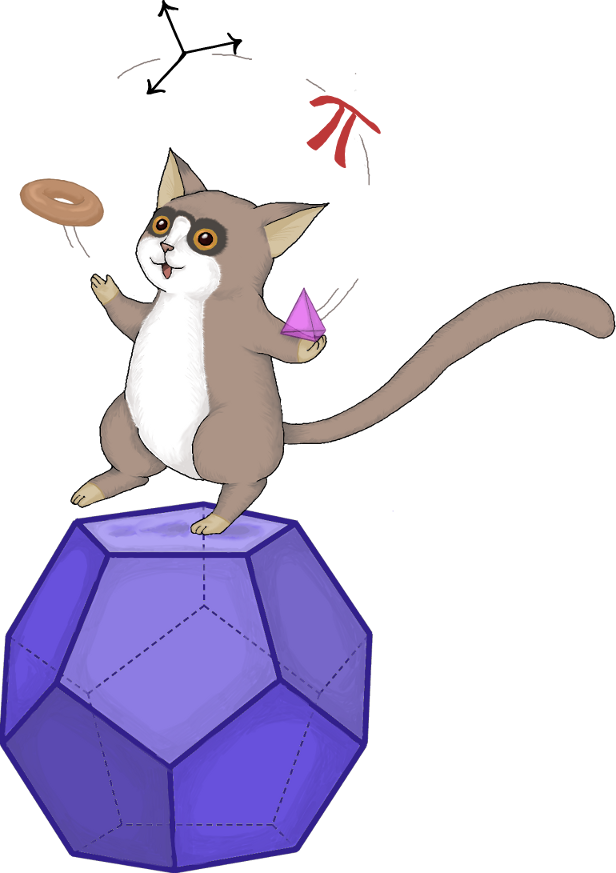
\includegraphics[scale=0.17]{cover}
}
\end{picture} 
	
\vspace{6em}

\begin{center}\Large{Mathe-Camp 2023}

\section*{Berechenbarkeit}\end{center}

\begin{defn}
	Ein \emph{Alphabet} $\Sigma$ ist eine endliche Menge von Buchstaben. Ein \emph{Wort} über einem solchen Alphabet ist eine endliche Folge von Buchstaben aus diesem Alphabet. Wir bezeichnet die Menge aller solcher Wörter mit $\Sigma^*$. Außerdem verwenden wir $\epsilon$ um das leere Wort zu beschreiben (also das Wort, das aus keinem Buchstaben besteht).
	
	Eine \emph{Sprache} $S$ über einem Alphabet $\Sigma$ ist eine (möglicherweise unendliche) Teilmenge $S \subseteq \Sigma^*$ (also eine Menge von Wörtern).
\end{defn}

\begin{defn}
	Sei $S$ eine Sprache über einem Alphabet $\Sigma^*$. Das zu $S$ gehörende \emph{Entscheidungsproblem} lautet dann:
	
	\underline{Eingabe:} Ein Wort $w \in \Sigma^*$
	
	\underline{Ausgabe:} Ja, falls $w \in S$, und nein, sonst
	
	Wir sagen, dass eine Sprache $S$ \emph{entscheidbar} ist, wenn es einen Algorithmus (ein Computerprogramm) gibt, dass das Entscheidungsproblem zu dieser Sprache löst.
\end{defn}

\begin{aufg}
	Wir betrachten die folgenden Sprachen:
	\begin{itemize}
		\item Die deutsche Sprache (im Sinn von: Die Menge aller Wörter, die um Duden stehen)
		\item Die Menge aller Palindrome (Wörter, die von vorne und hinten gelesen gleich sind)
		\item Die Menge aller natürlichen Zahlen
		\item Die Menge aller Terme aus natürlichen Zahlen sowie den Rechenzeichen $+$ und $-$
		\item Die Menge aller solcher Terme, die $0$ ergeben
		\item Die Menge aller solcher Terme, die zusätzlich auch Klammern enthalten dürfen und korrekt geklammert sind
		\item Die Menge aller natürlichen Zahlen in einer festen Menge $S \subseteq \IN$
		\item Die Menge aller Computerprogramme (in einer fest gewählten Programmiersprache, z.B. Python)
		\item Die Menge aller terminierenden Computerprogramme
	\end{itemize}
	Überlege dir jeweils, was ein geeignetes Alphabet für diese Sprachen ist.
	
	Was denkst du: Welche dieser Sprachen ist entscheidbar?
\end{aufg}

\begin{beob}
	Wenn eine Sprache entscheidbar ist, ist klar wie wir das beweisen können: Wir müssen einfach nur ein entsprechendes Programm angeben (wobei es natürlich unter Umständen sehr schwer ist, so ein Programm zu finden).
	
	Aber wie können wir zeigen, dass eine Sprache unentscheidbar ist? Dafür müssen wir zeigen, dass es kein Programm geben kann, das diese Sprache entscheidet. Das klingt nach einer sehr schweren Aufgabe!
\end{beob}

Im Folgenden wollen wir nun verschiedene Modelle für Computer kennenlernen und verstehen, was diese jeweils können (und nicht können).

\section{Endliche Automaten}

Ein endlicher Automat funktioniert grob gesprochen wie folgt: Er liest ein Eingabewort Buchstabe für Buchstabe ein und sagt am Ende entweder Ja oder Nein. Dazu hat der Automat eine endliche Menge von Zustanden zwischen denen er während dem Einlesen hin und her wechseln kann. Die Ausgabe am Ende hängt davon ab, in welchem Zustand sich der Automat am Ende befindet.

Solche endlichen Automaten kann man gut als gerichtete Graphen darstellen, zum Beispiel:
\begin{center}
	\begin{tikzpicture}
		\node[draw,circle](0)at(0,0) {$q_0$};
		\node[draw,circle](1)at(3,1.5) {$q_1$};
		\node[draw,circle,double](2)at(3,-1.5) {$q_2$};
		\node[draw,circle,double](3)at(6,0) {$q_3$};
		
		\draw[thick,<-](0) -- +(-1,0);
		\draw[thick,->](0) --node[above,sloped]{$a$} (1);
		\draw[thick,->](0) to[bend left=20] node[above,sloped]{$b$} (2);
		\draw[thick,->](0) to[bend right=20] node[below,sloped]{$c$} (2);
		\draw[thick,->](1) -- node[right]{$b$} (2);
		\draw[thick,->](2) -- node[below,sloped]{$c$} (3);
		
		\draw[thick,->](1) to[out=110,in=70,looseness=10] node[above]{$a$} (1);
		\draw[thick,->](2) to[out=-110,in=-70,looseness=10] node[below]{$b$} (2);
	\end{tikzpicture}
\end{center}

Hierbei sind $q_0, q_1, q_2, q_3$ die \emph{Zustände} des Automaten, $q_0$ ist der Startzustand und $q_2$ und $q_3$ sind die (akzeptierenden) Endzustände. Der Automat funktioniert nun wie folgt: Er beginnt im Startzustand $q_0$ und liest den ersten Buchstaben des Eingabewortes. Dann läuft es entlang einer Kante, auf der dieser Buchstabe steht, zum nächsten Zustand und wiederholt den Vorgang hier mit dem zweiten Buchstaben des Wortes. Kommt der Automat in einen Zustand, von dem aus es keine ausgehende Kante mit dem aktuellen Buchstaben gibt, so verwirft er das Wort (antwortet also mit Nein). Schafft er es das Wort bis zum Ende zu lesen, so antwortet er mit Ja, falls er sich in diesem Moment in einem Endzustand befindet, und mit Nein sonst.

\begin{bsp}
	Wir legen unserem Automaten das Wort $aabc$ vor. Der Automat liest den ersten Buchstaben ($a$) und wechselt zum Zustand $q_1$. Der Automat liest den zweiten Buchstaben ($a$) und landet erneut im Zustand $a$. Danach liest es den dritten Buchstaben ($b$) und wechselt in den Zustand $q_2$ und schließlich den letzten Buchstaben ($c$) und wechselt in den Zustand $q_3$. Da dies ein Endzustand (und das Wort zu Ende) ist, antwortet der Automat mit Ja.
\end{bsp}

\begin{aufg}
	Welche der folgenden Worte akzeptiert unser Automat:
		\[b,\quad cbb,\quad aaa,\quad aab,\quad aac,\quad cc\]
\end{aufg}

Mit etwas Überlegen erkennen wir, dass die Sprache aller Wörter, die dieser Automat akzeptiert wie folgt lautet:
	\[\{a^nb^m, a^nb^mc, b^n, b^nc, cb^k, cb^kc \,|\, mn \geq 1, k \geq 0\}\]
Hierbei steht beispielsweise $a^nb^m$ für das Wort, das aus $n$ $a$s gefolgt von $m$ $b$s besteht. Also zum Beispiel $a^3b^5 = aaabbbbb$.

\begin{aufg}
	Welche der folgenden Sprachen über dem Alphabet $\{a,b,c\}$ kann von einem endlichen Automaten entschieden werden?
	\begin{itemize}
		\item Alle Wörter, die mit $a$ beginnen und mindestens ein $b$ enthalten.
		\item Alle Wörter, die nicht mit $c$ enden.
		\item Alle Wörter, die mit $aa$ beginnen und mit $b$ enden.
		\item Alle Wörter, die genau zwei $b$ enthalten.
		\item Alle Wörter, die eine durch $3$ teilbare Anzahl an $a$ enthalten.
		\item Die Sprache $\{\epsilon,ab,aabb,aaabbb\}$.
		\item Die Sprache $\{a^kb^k | k \geq 0\}$.
	\end{itemize}
\end{aufg}

Wie können wir beweisen, dass eine Sprache von keinem endlichen Automaten entschieden werden kann? Eine Antwort hierauf liefert das Pumping-Lemma:

\begin{lemma}
	Sei $M$ ein endlicher Automat und $S$ die von ihm entschiedene Sprache. Dann gibt es eine natürliche Zahl $n \in \IN$ mit der folgenden Pumping-Eigenschaft:
	
	Für jedes Wort $w \in S$ aus $n$ oder mehr Buchstaben gibt es eine Zerlegung von $w$ in drei Teilworte $u$, $v$ und $x$, sodass $uv$ höchstens $n$ Buchstaben enthält, $v$ mindestens einen Buchstaben und für jedes $i \in \INo$ auch das Wort $uv^ix$ zur Sprache $S$ gehört. 
	
	Oder in Formeln:
		\[\exists n \in \IN: \forall w \in S: \abs{w} \geq n \implies \exists u,v,x \in \Sigma^*: w=uvx, \abs{uv} \leq n, \abs{v} \geq 1, \forall i \in \INo: uv^ix \in S.\]
\end{lemma}

\begin{proof}[Beweisidee]
	Wähle als $n$ die Anzahl der Zustände von $M$. Lesen wir ein Wort $w$ der Länge $n$ oder mehr ein, so muss $M$ nach dem Einlesen der ersten $n$ Buchstaben mindestens einen Zustand doppelt besuchen (Schubfachprinzip!). Sei $q$ dieser Zustand. Dann definieren wir $u$ als den Teil von $w$, den $M$ gelesen hat als es $q$ zum ersten Mal besucht, $v$ als den Teil bis zum nächsten Besuch von $q$ und $z$ als den Rest. Man kann sich nun überlegen, dass diese Zerlegung alle gewünschten Eigenschaften erfüllt.
\end{proof}

Anschaulich gesprochen besagt, dass Pumping-Lemma, dass in jeder Sprache, die von einem endlichen Automaten entschieden wird, alle ausreichend langen Worte ein Mittelstück besitzen, dass man beliebig oft auf- oder abpumpen kann.

Für sich genommen ist das keine besonders interessante Eigenschaft. Wir können sie aber dazu nutzen, um zu zeigen, dass eine gegebene Sprache nicht von einem endlichen Automaten entschieden werden kann: Dazu müssen wir nur zeigen, dass diese Sprache die obige Pumping-Eigenschaft nicht hat.

\begin{aufg}
	Zeige mit Hilfe des Pumping-Lemmas, dass es für folgende Sprachen keinen endlichen Automaten gibt:
	\begin{itemize}
		\item $\{a^kb^k | k \geq 0 \}$
		\item $\{a^mb^k | k \geq m \geq 0 \}$
		\item $\{a^mb^k | m \geq k \geq 0 \}$
		\item $\{a^{k^2} | k \geq 0 \}$
	\end{itemize}
\end{aufg}

\begin{zaufg}
	Untersuche, ob die folgenden beiden Sprachen von einem endlichen Automaten entschieden werden können:
	\begin{enumerate}[label=\alph*)]
		\item Die Sprache aller Wörter aus $a$ und $b$, in denen die Buchstabenfolge $ab$ und $ba$ gleich oft vorkommen.
		\item $S \coloneqq \{a^p | p \text{ Primzahl}\}$
		
		\textit{Hinweis:} Zahlen der Form $n!+2$ könnten hier hilfreich sein.		
	\end{enumerate}
\end{zaufg}

\begin{zaufg}
	Ein \emph{un}endlicher Automat ist ein Automat, der genauso funktioniert wie ein endlicher Automat, aber unendlich viele Zustände haben kann. Überlege dir, ob diese Automaten mächtiger sind als endliche Automaten. Gibt es Sprachen, die auch ein unendlicher Automat nicht entscheiden kann?
\end{zaufg}

\section{Abschlusseigenschaften}

\begin{lemma}\label{lemma:EAAbschlusseigenschaften}
	Seien $S_1$ und $S_2$ zwei Sprachen über einem gemeinsamen Alphabet $\Sigma$, die beide von einem endlichen Automaten entschieden werden. Dann werden auch die folgenden Sprachen von einem endlichen Automaten entschieden:
	\begin{itemize}
		\item $S_1 \cap S_2$
		\item $S_1 \cup S_2$
		\item $\Sigma^* \setminus S_1$
	\end{itemize}
\end{lemma}

\begin{proof}[Beweisidee]
	Seien $M_1$ und $M_2$ zwei endliche Automaten für $S_1$ und $S_2$. Für die ersten beiden Sprachen verwenden wir den sogenannten Produktautomaten: Dieser hat einen Zustand $(q,p)$ für jeden Zustand $q$ von $M_1$ und Zustand $p$ von $M_2$. Es gibt nun einen Übergang $a$ von $(q,p)$ nach $(q',p')$ falls $M_1$ einen Übergang $a$ von $q$ nach $q'$ hat und $M_2$ einen Übergang $a$ von $p$ nach $p'$. Für die erste Sprache ist ein Zustand $(q,p)$ akzeptierend, falls sowohl $q$ als auch $p$ akzeptierend sind. Für die zweite Sprache, falls mindestens $q$ oder $p$ akzeptierend sind.
	
	Für die dritte Sprache überlegen wir uns, dass es leicht möglich ist $M_1$ so zu erweitern, dass es jedes Wort komplett einlesen kann (also nie stecken bleibt). Dann genügt es akzeptierende und nicht-akzeptierende Zustände zu vertauschen.
\end{proof}

\begin{zaufg}
	Wir betrachten die Sprache
		\[\{a^mb^kc^k | m,k \geq 1\} \cup \{b^mc^k | m,k \geq 0\}.\]
	Diese Sprache kann von keinem endlichen Automaten entschieden werden.
	\begin{enumerate}[label=\alph*)]
		\item Warum können wir das nicht mit Hilfe des Pumping-Lemmas zeigen?
		\item Verwende eine geeignete Abschlusseigenschaft um diese Aussage zu zeigen.
	\end{enumerate}
\end{zaufg}

\begin{beob}
	Diese Aufgabe zeigt also, dass das Pumping-Lemma keine vollständige Charakterisierung der durch endliche Automaten entschiedenen Sprachen liefert. Insbesondere kann es also vorkommen, dass eine Sprache die Pumping-Eigenschaft hat und trotzdem nicht von einem endlichen Automaten entschieden werden kann.
\end{beob}

\section{Nichtdeterministische endliche Automaten}

Bisher haben wir nur sogenannte \emph{deterministische} endliche Automaten betrachtet. Das heißt für jedes feste Eingabe Wort gibt es nur einen Weg wie der Automat dieses einlesen kann. Insbesondere bedeutet das, dass jeder Zustand nur höchstens eine ausgehende Kante zu jedem Buchstaben des Alphabets haben darf.

\begin{defn}
	Ein \emph{nichtdeterministischer endlicher Automat} ist ein endlicher Automat, bei dem Zustände mehrere ausgehende Kanten mit dem gleichen Buchstaben haben dürfen. Außerdem kann es $\epsilon$-Kanten geben. Das sind Kanten, über die der Automat den Zustand wechseln kann ohne dabei einen Buchstaben einzulesen.
	
	Ein nichtdeterministischer endlicher Automat akzeptiert ein Eingabewort, wenn es wenigstens einen Weg gibt dieses Wort einzulesen und in einem akzeptierenden Zustand zu enden.
\end{defn}

\begin{aufg}
	Betrachte den folgenden nicht-deterministischen Automaten:
	\begin{center}
		\begin{tikzpicture}
			\node[draw,circle](0)at(0,0) {$q_0$};
			\node[draw,circle](1)at(3,0) {$q_1$};
			\node[draw,circle,double](2)at(6,0) {$q_2$};
			\node[draw,circle](3)at(3,-3) {$q_3$};
			
			\draw[thick,<-](0) -- +(-1,0);
			\draw[thick,->](0) to[bend left] node[above,sloped]{$a$} (1);
			\draw[thick,->](1) to[bend left] node[below,sloped]{$b$} (0);
			\draw[thick,->](1) -- node[above,sloped]{$b$} (2);
			\draw[thick,->](1) -- node[right]{$a$} (3);
			\draw[thick,->](3) -- node[sloped,below]{$\epsilon$} (2);
			\draw[thick,->](3) -- node[sloped,below]{$a$} (0);
		\end{tikzpicture}
	\end{center}
	Welche Sprache entscheidet dieser Automat?
\end{aufg}

Die Akzeptanzbedingung von nichtdeterministischen Automaten kann man so interpretieren, dass der Automat beim Einlesen immer richtig rät, wann immer er mehrere Möglichkeiten zur Auswahl hat. Das klingt nun so als wären nichtdeterministische endliche Automaten deutlich mächtiger als deterministische. Überraschenderweise ist das aber nicht der Fall:

\begin{lemma}
	Sei $S$ eine Sprache, die von einem nichtdeterministischen endlichen Automaten entschieden wird. Dann gibt es auch einen deterministischen endlichen Automaten, der diese Sprache entscheidet.
\end{lemma}

\begin{proof}[Beweisidee]
	Das Vorgehen hier ist ähnlich wie für \Cref{lemma:EAAbschlusseigenschaften} nur, dass wir diesmal die Potenzmenge der Zustandsmenge als neue Zustandsmenge verwenden.
\end{proof}

\begin{aufg}
	Wandle den nichtdeterministischen Automaten aus der vorherigen Aufgabe in einen deterministischen um.
\end{aufg}

\begin{aufg}
	Seien $S_1$ und $S_2$ zwei Sprachen, die von einem endlichen Automaten entschieden werden. Dann kann auch die folgende Sprache von einem endlichen Automaten entschieden werden:
		\[S_1\cdot S_2 \coloneqq \{ww' \,|\, w \in S_1, w' \in S_2\}.\]
\end{aufg}

\section{Kellerautomaten}

Ein Problem von endlichen Automaten ist, dass sie nicht (beliebig) zählen können. Das liegt daran, dass sie keinen wirklichen Speicher haben (außer den endlich vielen Zuständen). Wir wollen unsere Automaten daher jetzt um einen einfachen Speicher erweitern: Einen \emph{Keller} (oder auch \emph{Stack}).

\begin{defn}
	Ein Kellerautomat funktioniert im Wesentlichen wie ein endlicher Automat, hat aber zusätzlich Zugriff auf einen Keller. Dieser Keller enthält zu Beginn nur ein einziges Symbol $\bot$, welches nicht Teil des Eingabealphabets ist. Bei einem Übergang von einem Zustand zum nächsten liest ein Kellerautomat jetzt nicht nur den aktuellen Buchstaben des Eingabewortes, sondern auch das oberste Symbol im Keller. Danach löscht er dieses Symbol aus dem Keller und fügt eine beliebige (endliche!) Anzahl von neuen Buchstaben oben im Keller hinzu (insbesondere ist es auch erlaubt kein Symbol hinzuzufügen oder das gerade gelöschte Symbol wieder hinzuzufügen).
\end{defn}

Einen Kellerautomat können wir nun wie folgt darstellen:
\begin{center}
	\begin{tikzpicture}
		\node[draw,circle](0)at(0,0) {$q_0$};
		\node[draw,circle](1)at(3,0) {$q_1$};
		\node[draw,circle](2)at(6,0) {$q_2$};
		\node[draw,circle,double](3)at(9,0) {$q_3$};
		
		\draw[thick,<-](0) -- +(-1,0);
		\draw[thick,->](0) --node[above]{$a,\bot,\bot a$} (1);
		\draw[thick,->](1) --node[above]{$b,a,\epsilon$} (2);
		\draw[thick,->](2) -- node[above]{$\epsilon,\bot,\epsilon$} (3);
		
		\draw[thick,->](1) to[out=-110,in=-70,looseness=10] node[below]{$a,a,aa$} (1);
		\draw[thick,->](2) to[out=-110,in=-70,looseness=10] node[below]{$b,a,\epsilon$} (2);
	\end{tikzpicture}
\end{center}
Auf den Kanten stehen nun immer drei Dinge: Der gelesene Buchstabe des Eingabewortes, der gelesene Buchstabe aus dem Keller und die Buchstaben die neu in den Keller gelegt werden (oder $\epsilon$, wenn nichts in den Keller gelegt wird).

\begin{aufg}
	Welche Sprache entscheidet der obige Kellerautomat?
\end{aufg}

Auch für die von Kellerautomaten entschiedenen Sprachen gibt es ein Pumping-Lemma:

\begin{lemma}
	Sei $S$ eine Sprache, die von einem Kellerautomaten entschieden wird. Dann gibt es eine Zahl $n \in \IN$ mit folgender Eigenschaft:
	
	Für jedes $w \in S$ mit $\abs{w} \geq n$ gibt es eine Zerlegung $w=uvxyz$, sodass $\abs{vxy} \leq n$, $\abs{vy} \geq 1$ und $uv^ixy^iz \in S$ für alle $i \in \INo$.
\end{lemma}

\begin{aufg}
	Welche der folgenden Sprachen kann von einem Kellerautomaten entschieden werden?
	\begin{itemize}
		\item Alle Wörter über dem Alphabet $\{a,b\}$ die gleich viele $a$ und $b$ enthalten.
		\item Alle Palindrome über einem festen Alphabet.
		\item $\{a^kb^kc^k | k \geq 0\}$
		\item Die Menge aller Wörter über dem Alphabet $\{(,)\}$, die einer korrekten Klammerung entsprechen.
	\end{itemize}
\end{aufg}

\begin{aufg}
	Finde zwei Sprachen $S_1$ und $S_2$ mit folgender Eigenschaft: Es gibt Kellerautomaten, die $S_1$ und $S_2$ entscheiden, aber keinen Kellerautomaten, der $S_1 \cap S_2$ entscheidet.
\end{aufg}

\begin{zaufg}
	Wir betrachten die Sprache aller Wörter der Form $wcw$, wobei $w$ ein beliebiges Wort aus den Buchstaben $a$ und $b$ sein kann. Gibt es einen Kellerautomaten, der diese Sprache entscheidet?
\end{zaufg}

\section{Turingmaschinen}

Eine Turingmaschine funktioniert ebenfalls ähnlich wie ein endlicher Automat, hat aber zwei zusätzliche Fähigkeiten:
\begin{itemize}
	\item Sie kann die Eingabe nicht nur einmal von links nach rechts lesen, sondern beim Lesen beliebig nach rechts und links springen.
	\item Sie kann die Eingabe nicht nur lesen, sondern auch überschreiben.
\end{itemize}

\begin{defn}
	Eine Turingmaschine startet mit einem unendlichen langen Band, auf dem zu Beginn das Eingabewort und sonst nur Leerzeichen (ein spezielles Symbol $\textvisiblespace$, welches nicht Teil des Eingabealphabets ist) stehen. Sie hat einen Schreib-/Lesekopf, der zu Beginn auf den ersten Buchstaben des Eingabewortes zeigt. Sie hat endlich viele Zustände, von denen einer ein Startzustand ist und einer oder mehrere ein akzeptierender Endzustand. Außerdem kann es auch verwerfende Endzustände geben. 
	
	Ein Übergang zwischen zwei Zuständen besteht aus drei Dingen: Lese den aktuellen Buchstaben vom Band, überschreibe diesen mit einem neuen Zustand und bewege den Kopf dann nach links oder rechts.
	
	Eine Turingmaschine akzeptiert ein Wort, wenn sie beim Einlesen des Wortes einen akzeptierenden Endzustand erreicht. Sie verwirft es, wenn sie einen verwerfenden Endzustand oder einen Zustand ohne geeignete ausgehende Kanten erreicht.
\end{defn}

\begin{beob}
	Beim Einlesen eines Wortes durch eine Turingmaschine können drei Dinge passieren:
	\begin{itemize}
		\item Das Wort wird akzeptiert.
		\item Das Wort wird verworfen.
		\item Die Berechnung der Turingmaschine endet nicht.
	\end{itemize}
\end{beob}

Eine Turingmaschine können wir wie folgt darstellen:
\begin{center}
	\begin{tikzpicture}
		\node[draw,circle](0)at(0,0) {$q_0$};
		\node[draw,circle](1)at(2,2) {$q_1$};
		\node[draw,circle](2)at(5,2) {$q_2$};
		\node[draw,circle](3)at(7,0) {$q_3$};
		\node[draw,circle](4)at(3.5,0) {$q_4$};
		\node[draw,circle](5)at(0,-3) {$q_5$};
		\node[draw,circle,double](6)at(0,-6) {$q_6$};
		
		\draw[thick,<-](0) -- +(-1,0);
		\draw[thick,->](0) --node[above,sloped]{$a,x,\rightarrow$} (1);
		\draw[thick,->](1) --node[above]{$c,c,\rightarrow$} (2);
		\draw[thick,->](2) -- node[above,sloped]{$\textvisiblespace,\textvisiblespace,\leftarrow$} (3);
		\draw[thick,->](3) -- node[above,sloped]{$b,\textvisiblespace,\leftarrow$} (4);
		\draw[thick,->](4) -- node[above,sloped]{$x,x,\rightarrow$} (0);
		\draw[thick,->](0) -- node[left]{$c,c,\rightarrow$} (5);
		\draw[thick,->](5) -- node[left]{$\textvisiblespace,\textvisiblespace,\leftarrow$} (6);
		
		\draw[thick,->](1) to[out=110,in=70,looseness=10] node[above]{$a,a,\rightarrow$} (1);
		\draw[thick,->](2) to[out=110,in=70,looseness=10] node[above]{$b,b,\rightarrow$} (2);
		\draw[thick,->](4) to[out=-110,in=-70,looseness=10] node[below,align=center]{$b,b,\leftarrow$\\$c,c,\leftarrow$\\$a,a,\leftarrow$} (4);
	\end{tikzpicture}
\end{center}

Auf den Kanten stehen hier der gelesene Buchstabe, der geschriebene Buchstabe und schließlich die Richtung, in die sich der Kopf danach bewegt.

\begin{aufg}
	Welche Wörter akzeptiert die obige Turingmaschine?
\end{aufg}

\begin{aufg}
	Finde eine Turingmaschine, die die Sprache $\{wcw | w \in \{a,b\}^*\}$ entscheidet.
\end{aufg}

\begin{aufg}
	Finde eine Turingmaschine, die auf manchen Eingaben nie hält.
\end{aufg}

\begin{zaufg}
	Finde eine Turingmaschine, die die Sprache $\{a^kb^kc^k | k \geq 0\}$ entscheidet.
\end{zaufg}

Die \emph{Churchsche These} besagt, dass eine Turingmaschine alles berechnen kann, was ein Algorithmus (Computerprogramm) berechnen kann. Eine solche Aussage kann man natürlich nicht beweisen. Bisher hat sie sich aber stets bewahrheitet. Insbesondere gilt sie also für alle bekannten Computermodelle und Programmiersprachen. Ein anderer interessanter Aspekt ist, dass eine Turingmaschine nicht mehr mächtiger wird, auch wenn wir ihr zusätzliche Fähigkeiten geben:

\begin{defn}
	Eine Mehrband-Turingmaschine funktioniert wie eine (Einband-)Turingmaschine hat aber mehrere (endlich viele!) Bänder zur Verfügung und einen Schreib-/Lesekopf pro Band. Für einen Zustandsübergang liest und schreibt die Maschine je einen Buchstaben mit jedem Kopf auf dessen jeweiligen Band und bewegt die Köpfe dann (unabhängig voneinander) nach links oder rechts.
\end{defn}

\begin{lemma}
	Alles, was eine Mehrband-Turingmaschine kann, können wir auch mit einer Einband-Turingmaschine machen.
\end{lemma}

\begin{zaufg}
	Eine Keller-Turingmaschine ist eine (Einband-)Turingmaschine, die zusätzlich einen Keller zur Verfügung hat (der genauso funktioniert wie bei einem Kellerautomaten).
	
	Zeige, dass eine Einband-Turingmaschinen alles können, was Keller-Turingmaschinen können.
\end{zaufg}

\begin{defn}
	Wir sagen, dass eine Turingmaschine $M$ eine Sprache $S$ \emph{entscheidet}, wenn sie genau die Wörter aus $S$ akzeptiert und alle anderen verwirft (und, insbesondere, also immer terminiert).
	
	Wir sagen dann auch, dass diese Sprache \emph{entscheidbar} ist.
\end{defn}

Ein interessantes Problem in der Betrachtung von Turingmaschinen ist das sogenannte \emph{Halteproblem}:

\underline{Eingabe:} Eine Turingmaschine $M$ und ein Wort $w$

\underline{Ausgabe:} Ja, falls $M$ bei Eingabe $w$ irgendwann hält, und Nein sonst

Wir fragen uns nun, ob es eine Turingmaschine gibt, die dieses Problem entscheidet. Etwas formaler fragen wir uns, ob die folgende Sprache durch eine Turingmaschine entscheidbar ist:
	\[\{\langle M, w\rangle \,|\, M \text{ ist eine Turingmaschine, die bei Eingabe von } w \text{ hält}\}\]
Dabei $\langle M, w\rangle$ eine geeignete Kodierung eines Tupels aus Turingmaschine und Eingabewort als Wort.

\begin{aufg}
	Es gibt eine Turingmaschine, die bei Eingabe von $\langle M, w\rangle$ die Turingmaschine $M$ auf dem Wort $w$ simuliert (also einfach genau das macht, was die Turingmaschine $M$ bei Eingabe von $w$ machen würde).
	
	Überlege dir, ob wir diese Turingmaschine verwenden können um das Halteproblem zu entscheiden.
\end{aufg}

\begin{satz}
	Das Halteproblem ist unentscheidbar.
\end{satz}

\begin{proof}[Beweisidee]
	Wir zeigen dies durch Widerspruch. Wir nehmen also an es gäbe eine Turingmaschine $H$, die das Halteproblem löst. Aus dieser können wir nun eine neue Turingmaschine $P$ konstruieren, die folgendes tut:
	
	Bei Eingabe eines Wortes $w$ prüft $P$ zunächst, ob $w$ die Kodierung einer Turingmaschine ist. Falls nicht, wird $w$ verworfen. Ansonsten sei $M$ diese Turingmaschine.
	
	Nun simuliert $P$ die Maschine $H$ um herauszufinden, ob $M$ bei Eingabe von $w = \langle M\rangle$ hält. Falls dem so ist, startet $P$ eine Endlosschleife. Ansonsten, akzeptiert $P$.
	
	Wir geben dieser Turingmaschine $P$ nun als Eingabewort ihre eigene Kodierung $\langle P\rangle$. Was passiert dann? Hält $P$ oder nicht? Eines davon muss passieren, wir stellen aber fest, dass beides zu einem Widerspruch führt. Also kann es die Turingmaschine $P$ nicht geben.
	
	Die einzige Annahme für unsere Konstruktion von $P$ war aber, dass es eine Turingmaschine $H$ gibt, die das Halteproblem löst. Also kann es eine solche Turingmaschine nicht geben.
\end{proof}

\begin{zaufg}
	Wir betrachten die Sprache aller Kodierungen von Turingmaschinen, die das Wort, das ihrer eigenen Kodierung entspricht, nicht akzeptieren.
	
	Zeige, dass diese Sprache unentscheidbar ist.
\end{zaufg}

\begin{zaufg}
	Da Turingmaschinen das Band auch beschreiben dürfen, kann man den Inhalt des Bandes am Ende der Berechnung auch als Ausgabe interpretieren. Wir können also auch Turingmaschinen bauen, die eine bestimmte Ausgabe haben.
	\begin{enumerate}[label=\alph*)]
		\item Konstruiere eine Turingmaschine, die als Eingabe eine Zahl in Binärdarstellung erhält und diese dann um eins erhöht.
		\item Konstruiere eine Turingmaschine, die zwei Zahlen (in Binärdarstellung) erhält und diese zusammen addiert.
	\end{enumerate}
	\textit{Hinweis:} Es macht die Beschreibung der Turingmaschinen evtl. einfacher, wenn du annimmst, dass sie mehrere Bänder haben. Du musst die Turingmaschine außerdem nicht zwangsläufig komplett formal angeben.
\end{zaufg}

\end{document}